\documentclass[10pt,a4paper]{article}
\usepackage[margin=21mm,headheight=15pt]{geometry}
\usepackage[T1]{fontenc}
\usepackage{lmodern,amsmath,amssymb,tikz,graphicx,hyperref,fancyhdr,enumitem}
\usetikzlibrary{arrows.meta,positioning,calc,decorations.pathmorphing}
\definecolor{ink}{RGB}{20,53,78}
\hypersetup{colorlinks=true,urlcolor=ink,linkcolor=ink}
\setlength{\parindent}{0pt}\setlength{\parskip}{5pt}
\emergencystretch=3em
\pagestyle{fancy}\fancyhf{}\fancyfoot[C]{\thepage}
\renewcommand{\headrulewidth}{.3pt}
\newcommand{\task}[2]{\par\medskip{\color{ink}\Large\bfseries #1. #2}\par\smallskip}
\newcommand{\answer}{\par\smallskip\textbf{Worked reasoning.} }
\setlist[enumerate]{label=\textbf{(\alph*)},leftmargin=7mm,itemsep=7pt}
\begin{document}
\fancyhead[L]{\small Control of Dynamical Systems}
\fancyhead[R]{\small Laboratory 04}
{\color{ink}\LARGE\bfseries Laboratory 04}\par
{\large A passive notch filter and component tolerance}\par
\textbf{Exercise sheet -- five integrated problems}\par
{\small\textbf{Evidence boundary.} Original hypothetical scenarios. Derive, calculate and justify decisions; every numerical record is synthetic. Figures are conceptual and not to scale.}
\smallskip\textbf{Shared nominal data.} Nominal series RLC network: $R=10\,\Omega$, $L=0.01$ H, $C=100\,\mu$F. Input is total applied voltage; output spans the combined inductor and capacitor. Components are ideal unless a part adds loss or tolerance.
\task{1}{Selecting the measured voltage in a real circuit}
A series RLC network is driven by an ideal voltage source. The probe spans the inductor and capacitor together, not the capacitor alone. Read the physical measurement terminals before writing the transfer.
\begin{center}\resizebox{\ifdim\width>.98\linewidth.98\linewidth\else\width\fi}{!}{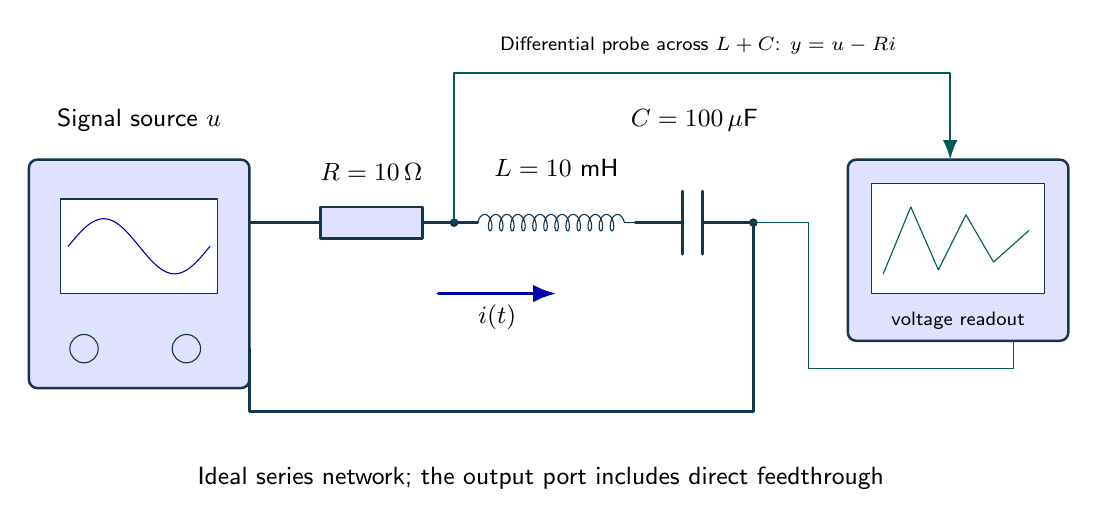
\begin{tikzpicture}[
font=\sffamily\small,>=Latex,line cap=round,line join=round,
wall/.style={draw=ink,line width=1.2pt,fill=blue!5},
water/.style={fill=cyan!25,draw=none},
metal/.style={draw=ink,fill=blue!12,line width=.9pt},
flow/.style={->,draw=blue!65!black,line width=1.2pt},
heat/.style={->,draw=orange!85!black,line width=1.1pt},
measure/.style={->,draw=teal!70!black,line width=.9pt},
dim/.style={<->,draw=ink!65,line width=.6pt},
spring/.style={draw=ink,decorate,decoration={coil,aspect=.5,segment length=4pt,amplitude=3pt}},
wire/.style={draw=ink,line width=1pt},
lab/.style={align=center,font=\sffamily\small},
smalllab/.style={align=center,font=\sffamily\scriptsize}]

\draw[metal,rounded corners=3pt](.3,1.1)rectangle(3.1,4);
\draw[fill=white,draw=ink](.7,2.3)rectangle(2.7,3.5);
\draw[blue!70!black,domain=.8:2.6,samples=60]plot(\x,{2.9+.35*sin(360*(\x-.8)/1.8)});
\draw[ink](1,1.6)circle(.18)(2.3,1.6)circle(.18);
\node[lab]at(1.7,4.5){Signal source $u$};
\draw[wire](3.1,3.2)--(4,3.2);
\draw[metal](4,3)rectangle(5.3,3.4);
\node[lab]at(4.65,3.85){$R=10\,\Omega$};
\draw[wire](5.3,3.2)--(6,3.2);
\draw[spring](6,3.2)--(8,3.2);
\draw[wire](8,3.2)--(8.6,3.2);
\draw[wire](8.6,2.8)--(8.6,3.6)(8.85,2.8)--(8.85,3.6);
\draw[wire](8.85,3.2)--(9.5,3.2)--(9.5,.8)--(3.1,.8)--(3.1,1.6);
\node[lab]at(7,3.9){$L=10$ mH};
\node[lab]at(8.75,4.5){$C=100\,\mu$F};
\draw[flow](5.5,2.3)--(7,2.3)node[midway,below]{$i(t)$};
\draw[metal,rounded corners=3pt](10.7,1.7)rectangle(13.5,4);
\draw[fill=white,draw=ink](11,2.3)rectangle(13.2,3.7);
\draw[teal!70!black](11.15,2.55)--(11.5,3.4)--(11.85,2.6)--(12.2,3.3)--(12.55,2.7)--(13,3.1);
\node[smalllab]at(12.1,1.95){voltage readout};
\fill[ink](5.7,3.2)circle(.055)(9.5,3.2)circle(.055);
\draw[measure](5.7,3.2)--(5.7,5.1)--(12,5.1)--(12,4);
\draw[teal!70!black](9.5,3.2)--(10.2,3.2)--(10.2,1.35)--(12.8,1.35)--(12.8,1.7);
\node[smalllab]at(8.8,5.45){Differential probe across $L+C$: $y=u-Ri$};
\node[lab]at(6.8,-.05){Ideal series network; the output port includes direct feedthrough};
\end{tikzpicture}
}\par{\small A source excites the series RLC network; an ideal differential probe spans the combined inductor and capacitor. Measuring only the capacitor would produce a different transfer function. Wire placement is schematic.}\end{center}
\begin{enumerate}
\item A voltage source drives series $R=10\,\Omega$, $L=0.01$ H and $C=100\,\mu$F. Output is the sum of inductor and capacitor voltages. Derive $H(s)$ and its DC and high-frequency gains.
\item Find the notch frequency, damping ratio, poles and zeros for the nominal circuit. State whether a zero on the imaginary axis makes the circuit internally unstable.
\item Derive the capacitor-voltage transfer for the same components and compare its numerator and direct feedthrough with those of the specified combined output. Explain why the poles remain unchanged.
\end{enumerate}
\vfill{\small\textbf{Submission.} Show the model, intermediate reasoning, units and a conclusion addressing the stated requirements.}

\newpage
\task{2}{A zero output with nonzero circulating energy}
Compare sinusoidal resonance with the response to a sudden voltage step. Both tests use the same passive network, but expose different aspects of the measured output.
\begin{enumerate}
\item At the notch frequency, the source has sinusoidal peak voltage 2 V. Find peak current, peak inductor and capacitor voltages, and the maximum energy in each reactive component.
\item Derive the nominal unit-step output. Find its initial and final values, and explain why neither contradicts rejection of a sinusoid at 1000 rad/s.
\item At sinusoidal resonance with a 2 V source peak, write magnetic and electric energy as functions of phase. Determine their sum and explain whether both energy maxima occur simultaneously.
\end{enumerate}
\vfill{\small\textbf{Submission.} Show the model, intermediate reasoning, units and a conclusion addressing the stated requirements.}

\newpage
\task{3}{When component tolerance and winding loss spoil the notch}
The ideal cancellation is challenged by a capacitor tolerance and a lossy inductor. Separate frequency detuning from an output floor caused by resistance.
\begin{center}\resizebox{\ifdim\width>.98\linewidth.98\linewidth\else\width\fi}{!}{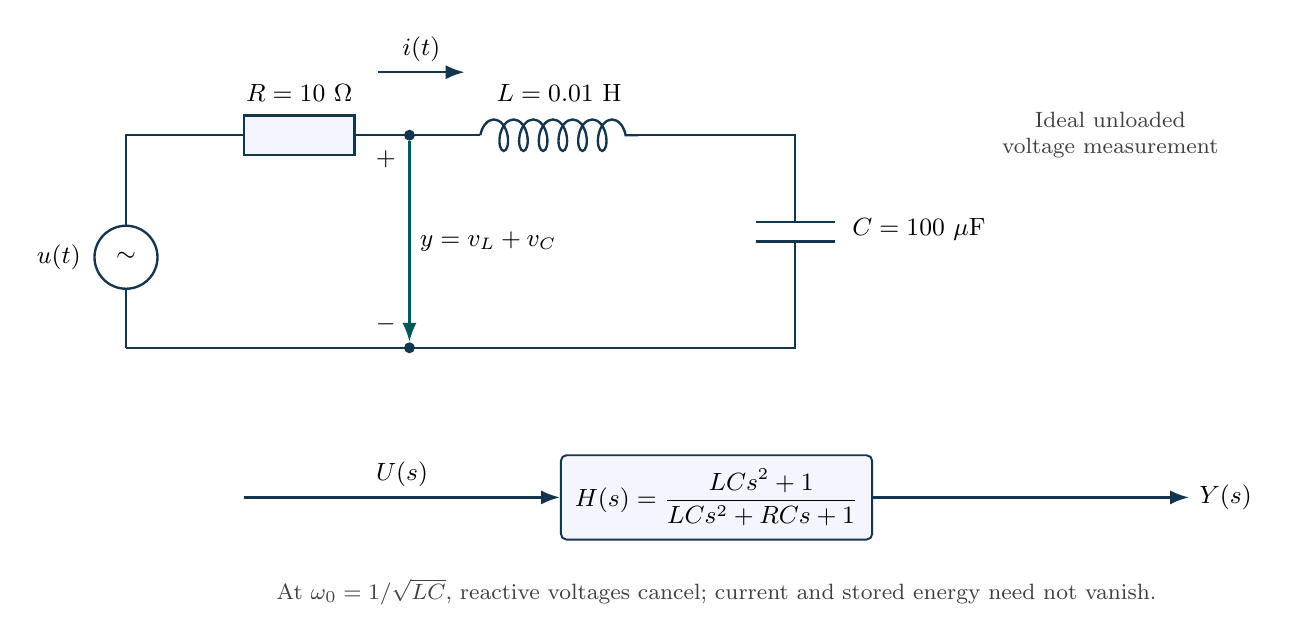
\begin{tikzpicture}[x=1cm,y=1cm,>=Latex,font=\small,
block/.style={draw=ink,fill=blue!4,rounded corners=2pt,minimum height=9mm,align=center,line width=.7pt,inner sep=5pt},
sum/.style={circle,draw=ink,fill=white,minimum size=6mm,inner sep=0pt,line width=.7pt},
sig/.style={->,draw=ink,line width=.85pt},
fb/.style={->,draw=teal!70!black,line width=.85pt},
dist/.style={->,draw=orange!75!black,line width=.85pt},
tap/.style={circle,fill=ink,inner sep=1.4pt},
note/.style={font=\footnotesize,align=center,text=black!75}]

\draw[draw=ink,line width=.85pt](.5,.3)--(.5,1.05);
\draw[draw=ink,line width=.85pt](.5,1.45)circle(.4);
\node at(.5,1.45){$\sim$};
\draw[draw=ink,line width=.85pt](.5,1.85)--(.5,3)--(2,3);
\node[left]at(.05,1.45){$u(t)$};
\draw[draw=ink,fill=blue!4,line width=.85pt](2,2.75)rectangle(3.4,3.25);
\node[above]at(2.7,3.3){$R=10\ \Omega$};
\draw[draw=ink,line width=.85pt](3.4,3)--(5,3);
\draw[decorate,decoration={coil,aspect=.55,segment length=2.5mm,amplitude=2mm},line width=.85pt,draw=ink](5,3)--(7,3);
\node[above]at(6,3.3){$L=0.01\ \mathrm{H}$};
\draw[draw=ink,line width=.85pt](7,3)--(9,3)--(9,1.9);
\draw[line width=.85pt,draw=ink](8.5,1.9)--(9.5,1.9)(8.5,1.65)--(9.5,1.65);
\draw[line width=.85pt,draw=ink](9,1.65)--(9,.3)--(.5,.3);
\node[right]at(9.6,1.8){$C=100\ \mu\mathrm{F}$};
\draw[sig](3.7,3.8)--node[above]{$i(t)$}(4.8,3.8);
\node[tap](a)at(4.1,3){};\node[tap](b)at(4.1,.3){};
\draw[fb](a)--node[right]{$y=v_L+v_C$}(b);
\node at(3.8,2.7){$+$};\node at(3.8,.6){$-$};
\node[note]at(13,3){Ideal unloaded\\voltage measurement};
\node[block](h)at(8,-1.6){$H(s)=\dfrac{LCs^2+1}{LCs^2+RCs+1}$};
\draw[sig](2,-1.6)--node[above]{$U(s)$}(h);
\draw[sig](h)--(14,-1.6)node[right]{$Y(s)$};
\node[note]at(8,-2.8){At $\omega_0=1/\sqrt{LC}$, reactive voltages cancel; current and stored energy need not vanish.};

\end{tikzpicture}
}\par{\small Series RLC network with output measured across L and C together. The output probe spans those two components, not the whole source.}\end{center}
\begin{enumerate}
\item With L and R fixed, let capacitance be 10 percent low or high. Calculate both notch frequencies. If the input remains at 1000 rad/s, give a formula for the residual output magnitude for a capacitance factor $f=C/C_0$.
\item Add winding resistance $r_L=1\,\Omega$ in series with the ideal inductor. The output spans that winding resistance, inductor and capacitor. Derive the new transfer and evaluate the output at the nominal resonant frequency.
\item At the nominal resonance, require output magnitude strictly below 0.05 when only winding resistance varies and $R=10\,\Omega$. Derive the permitted resistance interval and assess a 1 $\Omega$ winding.
\end{enumerate}
\vfill{\small\textbf{Submission.} Show the model, intermediate reasoning, units and a conclusion addressing the stated requirements.}

\newpage
\task{4}{Changing damping without moving the nominal notch}
The resistor can be changed without changing ideal L or C. Relate pole damping to the useful frequency interval of attenuation.
\begin{enumerate}
\item Choose R for critical damping without changing nominal L and C. Determine the resulting poles, and explain what happens to the ideal notch zeros.
\item Derive the two positive frequencies where the nominal magnitude is $1/\sqrt2$. Show that their product is $\omega_0^2$ and their separation is $R/L$.
\item Require a notch at 1000 rad/s, a half-power notch bandwidth of 800 rad/s and critically damped poles. Keep the nominal L and C and vary only R. Determine the resistance demanded by each requirement and decide whether all three can hold simultaneously.
\end{enumerate}
\vfill{\small\textbf{Submission.} Show the model, intermediate reasoning, units and a conclusion addressing the stated requirements.}

\newpage
\task{5}{A state model that preserves the circuit power balance}
Use the circuit states to connect frequency calculations to conservation of energy. Pay attention to the direct contribution of the applied voltage to the selected output.
\begin{enumerate}
\item For the nominal circuit, calculate output magnitude at 500 and 2000 rad/s. Explain the equality using the normalized frequency $r=\omega/\omega_0$.
\item Use capacitor voltage $v_C$ and current $i$ as states and input voltage $u$. Derive A, B, C and D for output equal to the ideal LC voltage sum. Explain the direct feedthrough term.
\item With states $[i,v_C]^T$, derive $\dot E$ for $E=Li^2/2+Cv_C^2/2$. Use it to distinguish passivity from the incorrect assertion that all output magnitudes must be below one.
\end{enumerate}
\vfill{\small\textbf{Submission.} Show the model, intermediate reasoning, units and a conclusion addressing the stated requirements.}

\end{document}
